\chapter{Transmisi Analog}
Dalam Bab 3, kita membahas keuntungan dan kerugian dari transmisi digital dan analog. Kami melihat bahwa meskipun transmisi digital sangat diinginkan, saluran low-pass diperlukan. Kami juga melihat bahwa transmisi analog adalah satu-satunya pilihan jika kami memiliki saluran bandpass. Transmisi digital telah dibahas dalam Bab 4; kita membahas transmisi analog dalam bab ini. 

Mengubah data digital menjadi sinyal analog bandpass. Secara tradisional disebut konversi digital-ke-analog. Mengubah sinyal analog low-pass menjadi sinyal analog bandpass secara tradisional disebut konversi analog-ke-analog. Dalam bab ini, kita membahas dua jenis konversi ini.

\section{Konversi Digital-to-Analog}
Digital-to-analog conversion is the process of changing one of the characteristics of an analog signal based on the information in digital data. Figure 5.1 shows the relationship between the digital information, the digital-to-analog modulating process, and the resultant analog signal.

\begin{figure}[htbp]
  \centering
  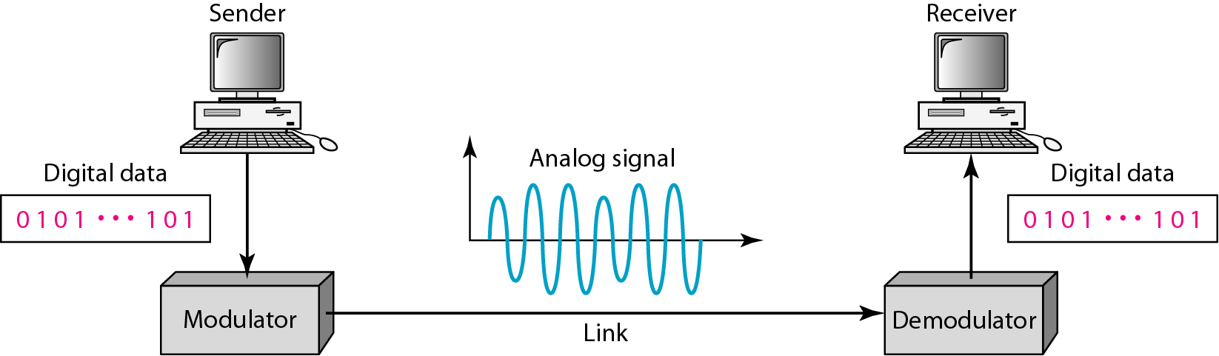
\includegraphics[width=0.9\columnwidth]{bab5/Picture1}
  \caption{Digital-to-analog conversion}
  \label{fig5:1}
\end{figure}

As discussed in Chapter 3, a sine wave is defined by three characteristics: amplitude, frequency, and phase. When we vary anyone of these characteristics, we create a different version ofthat wave. So, by changing one characteristic of a simple electric signal, we can use it to represent digital data. Any of the three characteristics can be altered in this way, giving us at least three mechanisms for modulating digital data into an analog signal: amplitude shift keying (ASK), frequency shift keying (FSK), and phase shift keying (PSK). In addition, there is a fourth (and better) mechanism that combines changing both the amplitude and phase, called quadrature amplitude modulation (QAM). QAM is the most efficient of these options and is the mechanism commonly used today (see Figure 5.2).

\begin{figure}[htbp]
  \centering
  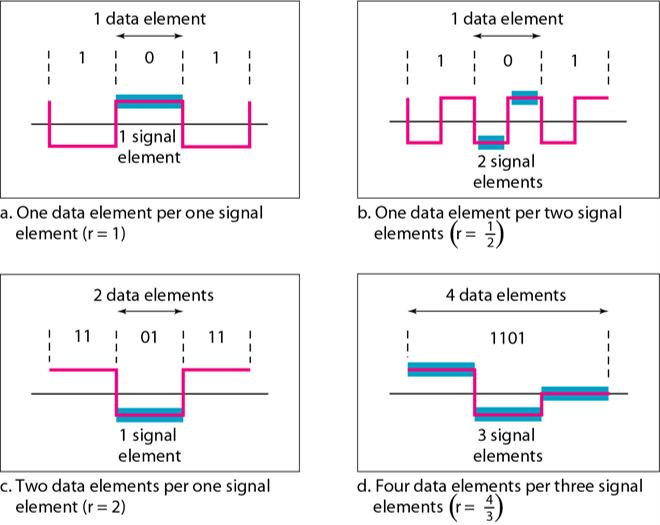
\includegraphics[width=0.9\columnwidth]{bab5/Picture2}
  \caption{Types of digital-to-analog conversion}
  \label{fig5:2}
\end{figure}

\subsection{Aspects of Digital-to-Analog Conversion}
Before we discuss specific methods of digital-to-analog modulation, two basic issues must be reviewed: bit and baud rates and the carrier signal

\subsection*{Data Element Versus Signal Element}
In Chapter 4, we discussed the concept of the data element versus the signal element. We defined a data element as the smallest piece of information to be exchanged, the bit. We also defined a signal element as the smallest unit of a signal that is constant. Although we continue to use the same terms in this chapter, we will see that the nature of the signal element is a little bit different in analog transmission.

\subsection*{Data Rate Versus Signal Rate}
We can define the data rate (bit rate) and the signal rate (baud rate) as we did for digital transmission. The relationship between them is

\begin{equation}
  S = N \times \frac{1}{r} \textnormal{ baud}
\end{equation}

where N is the data rate (bps) and r is the number of data elements carried in one signal element. The value of r in analog transmission is $r = log_2L$, where L is the type of signal element, not the level. The same nomenclature is used to simplify the comparisons.

Bit rate is the number of bits per second. Baud rate is the number of signal elements per second. In the analog transmission of digital data, the baud rate is less than or equal to the bit rate. The same analogy we used in Chapter 4 for bit rate and baud rate applies here. In transportation, a baud is analogous to a vehicle, and a bit is analogous to a passenger. We need to maximize the number of people per car to reduce the traffic.

\vspace{12pt}

\begin{example}
  An analog signal carries 4 bits per signal element. If 1000 signal elements are sent per second, find the bit rate.
  \label{example5:1}
\end{example}

\begin{solution}
  In this case, r = 4, S = 1000, and N is unknown. We can find the value of N from

  \begin{equation*}
    S = N \times \frac{1}{r} \quad \textnormal{ or } \quad N = S \times r = 1000 \times 4 = 4000 \textnormal{ bps}
  \end{equation*}
\end{solution}

\vspace{12pt}

\begin{example}
  An analog signal has a bit rate of 8000 bps and a baud rate of 1000 baud. How many data elements are carried by each signal element? How many signal elements do we need?
  \label{example5:2}
\end{example}

\begin{solution}
  In this example, S = 1000, N =8000, and rand L are unknown. We find first the value of rand then the value of L.

  \begin{align*}
    S &= N \times \frac{1}{r} \quad \textnormal{ } \textnormal{ } \Longrightarrow \quad r = \frac{N}{S} = \frac{8000}{1000} = 8 \textnormal{ bit/baud} \\
    r &= log_2L \quad \quad \Longrightarrow \quad L = 2^r = 2^8 = 256
  \end{align*}
\end{solution}

\subsection*{Bandwidth}
The required bandwidth for analog transmission of digital data is proportional to the signal rate except for FSK, in which the difference between the carrier signals needs to be added. We discuss the bandwidth for each technique.

\subsection*{Carrier Signal}
In analog transmission, the sending device produces a high-frequency signal that acts as a base for the information signal. This base signal is called the carrier signal or carrier frequency. The receiving device is tuned to the frequency of the carrier signal that it expects from the sender. Digital information then changes the carrier signal by modifying one or more of its characteristics (amplitude, frequency, or phase). This kind of modification is called modulation (shift keying).

\subsection{Amplitude Shift Keying}
In amplitude shift keying, the amplitude of the carrier signal is varied to create signal elements. Both frequency and phase remain constant while the amplitude changes.

\subsection*{Binary ASK (BASK)}
Although we can have several levels (kinds) of signal elements, each with a different amplitude, ASK is normally implemented using only two levels. This is referred to as binary amplitude shift keying or on-off keying (OOK). The peak amplitude of one signal level is 0; the other is the same as the amplitude of the carrier frequency. Figure 5.3 gives a conceptual view of binary ASK.

\begin{figure}[htbp]
  \centering
  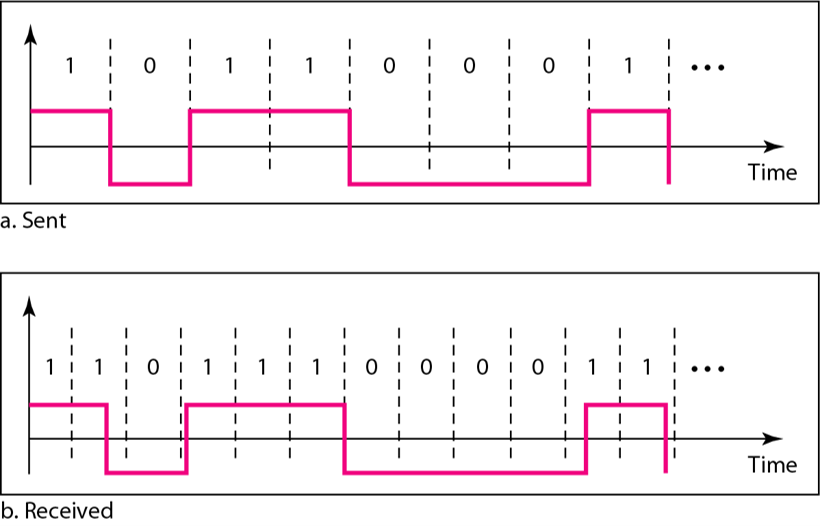
\includegraphics[width=0.9\columnwidth]{bab5/Picture3}
  \caption{Binary amplitude shift keying}
  \label{fig5:3}
\end{figure}

Bandwidth for ASK Figure 5.3 also shows the bandwidth for ASK. Although the carrier signal is only one simple sine wave, the process of modulation produces a nonperiodic composite signal. This signal, as was discussed in Chapter 3, has a continuous set of frequencies. As we expect, the bandwidth is proportional to the signal rate (baud rate). However, there is normally another factor involved, called d, which depends on the modulation and filtering process. The value of d is between 0 and 1. This means that the bandwidth can be expressed as shown, where 5 is the signal rate and the B is the bandwidth

\begin{equation}
  B = (1 + d) \times S
\end{equation}

The formula shows that the required bandwidth has a minimum value of 5 and a maximum value of 25. The most important point here is the location of the bandwidth. The middle of the bandwidth is where Ie the carrier frequency, is located. This means if we have a bandpass channel available, we can choose our Ie so that the modulated signal occupies that bandwidth. This is in fact the most important advantage of digital-to-analog conversion. We can shift the resulting bandwidth to match what is available

\textbf{Implementation} The complete discussion of ASK implementation is beyond the scope of this book. However, the simple ideas behind the implementation may help us to better understand the concept itself. Figure 5.4 shows how we can simply implement binary ASK.

If digital data are presented as a unipolar NRZ (see Chapter 4) digital signal with a high voltage of I V and a low voltage of 0 V, the implementation can achieved by multiplying the NRZ digital signal by the carrier signal coming from an oscillator. When the amplitude of the NRZ signal is 1, the amplitude of the carrier frequency is held; when the amplitude of the NRZ signal is 0, the amplitude of the carrier frequency IS zero.

\begin{figure}[htbp]
  \centering
  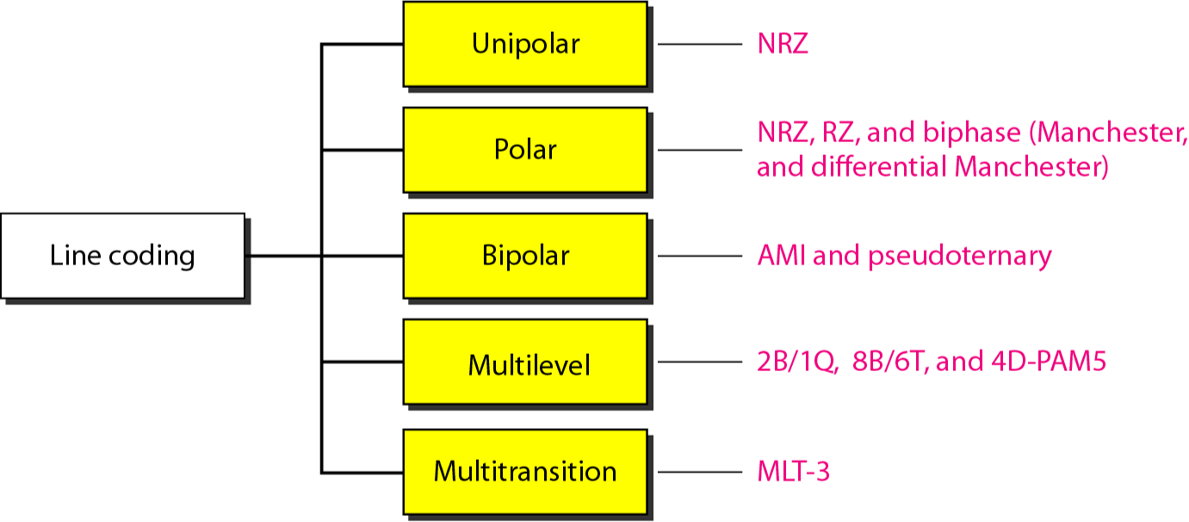
\includegraphics[width=0.9\columnwidth]{bab5/Picture4}
  \caption{Implementation of binary ASK}
  \label{fig5:4}
\end{figure}

\vspace{12pt}

\begin{example}
  We have an available bandwidth of 100 kHz which spans from 200 to 300 kHz. What are the carrier frequency and the bit rate if we modulated our data by using ASK with d =I?
  \label{example5:3}
\end{example}

\begin{solution}
  The middle of the bandwidth is located at 250 kHz. This means that our carrier frequency can be atfe =250 kHz. We can use the formula for bandwidth to find the bit rate (dengan d = 1, r = 1)

  \begin{equation*}
    B = (1 + d) \times S = 2 \times N \times \frac{1}{r} = 2 \times N = 100 \textnormal{ kHz} \quad \Longrightarrow \quad N = 500 \textnormal{ kbps}
  \end{equation*}
\end{solution}

\vspace{12pt}

\begin{example}
  In data communications, we normally use full-duplex links with communication in both directions. We need to divide the bandwidth into two with two carrier frequencies, as shown in Figure 5.5. The figure shows the positions of two carrier frequencies and the bandwidths.The available bandwidth for each direction is now 50 kHz, which leaves us with a data rate of 25 kbps in each direction.
  \label{example5:4}
\end{example}

\begin{figure}[htbp]
  \centering
  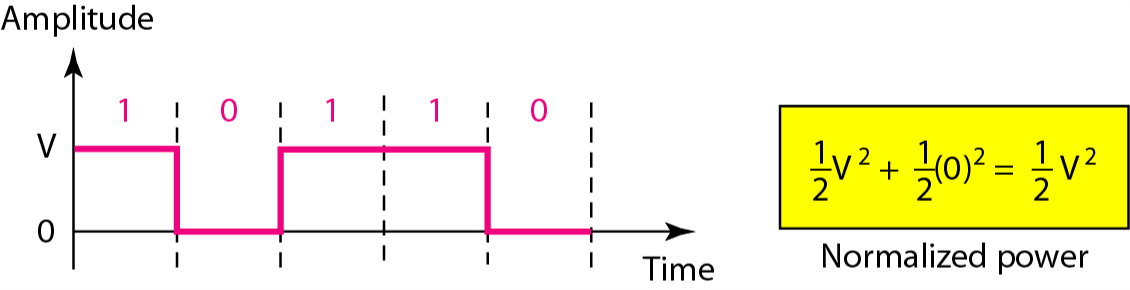
\includegraphics[width=0.9\columnwidth]{bab5/Picture5}
  \caption{Bandwidth offull-duplex ASK used in Example 5.4}
  \label{fig5:5}
\end{figure}

\subsection*{Multilevel ASK}
The above discussion uses only two amplitude levels. We can have multilevel ASK in which there are more than two levels. We can use 4,8, 16, or more different amplitudes for the signal and modulate the data using 2, 3, 4, or more bits at a time. In these cases, r = 2, r = 3, r =4, and so on. Although this is not implemented with pure ASK, it is implemented with QAM (as we will see later).

\subsection{Frequency Shift Keying}
In frequency shift keying, the frequency of the carrier signal is varied to represent data. The frequency of the modulated signal is constant for the duration of one signal element, but changes for the next signal element if the data element changes. Both peak amplitude and phase remain constant for all signal elements.

\subsection*{Binary FSK (BFSK)}
One way to think about binary FSK (or BFSK) is to consider two carrier frequencies. In Figure 5.6, we have selected two carrier frequencies, f1 and f2. We use the first carrier if the data element is 0; we use the second if the data element is 1. However, note that this is an unrealistic example used only for demonstration purposes. Normally the carrier frequencies are very high, and the difference between them is very small.

\begin{figure}[htbp]
  \centering
  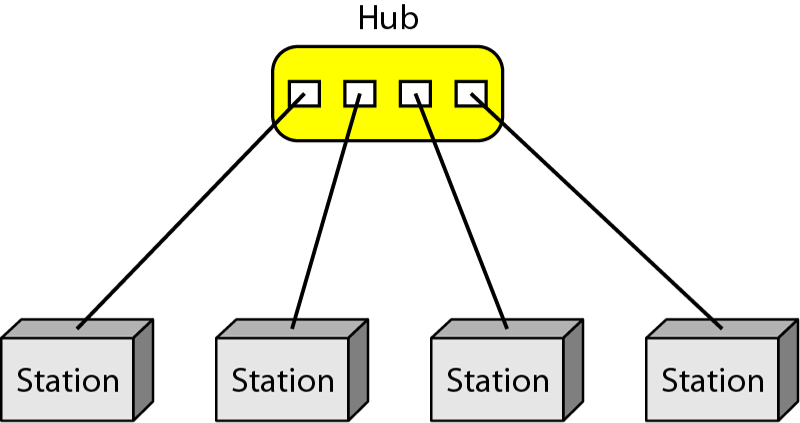
\includegraphics[width=0.9\columnwidth]{bab5/Picture6}
  \caption{Binary frequency shift keying}
  \label{fig5:6}
\end{figure}

As Figure 5.6 shows, the middle of one bandwidth isJI and the middle of the other ish. Both JI and12 are il/ apart from the midpoint between the two bands. The difference between the two frequencies is 211f

Bandwidth for BFSK Figure 5.6 also shows the bandwidth of FSK. Again the carrier signals are only simple sine waves, but the modulation creates a nonperiodic composite signal with continuous frequencies. We can think of FSK as two ASK signals, each with its own carrier frequency Cil orh). If the difference between the two frequencies is 211j, then the required bandwidth is

\begin{equation}
  B = (1 + d) \times S + 2\Delta f
\end{equation}

What should be the minimum value of 211/? In Figure 5.6, we have chosen a value greater than (l + d)S. It can be shown that the minimum value should be at least S for the proper operation of modulation and demodulation

\begin{example}
  We have an available bandwidth of 100 kHz which spans from 200 to 300 kHz. What should be the carrier frequency and the bit rate if we modulated our data by using FSK with d =1?
\end{example}

\begin{solution}
  This problem is similar to Example 5.3, but we are modulating by using FSK. The midpoint of the band is at 250 kHz. We choose 2$\Delta$f to be 50 kHz; this means
  
  \begin{equation*}
    B = (1 + d) \times S + 2\Delta f = 100 \Longrightarrow 2S = 50 \textnormal{ kHz} \Longrightarrow S = 25 \textnormal{ kbaud}; N = 25 \textnormal{ kbps}
  \end{equation*}

  \noindent Compared to Example 5.3, we can see the bit rate for ASK is 50 kbps while the bit rate for FSK is 25 kbps.
\end{solution}

\textbf{Implementation} There are two implementations of BFSK: noncoherent and coherent. In noncoherent BFSK, there may be discontinuity in the phase when one signal element ends and the next begins. In coherent BFSK, the phase continues through the boundary of two signal elements. Noncoherent BFSK can be implemented by treating BFSK as two ASK modulations and using two carrier frequencies. Coherent BFSK can be implemented by using one voltage-controlled oscillator (VeO) that changes its frequency according to the input voltage. Figure 5.7 shows the simplified idea behind the second implementation. The input to the oscillator is the unipolar NRZ signal. When the amplitude of NRZ is zero, the oscillator keeps its regular frequency; when the amplitude is positive, the frequency is increased.

\begin{figure}[htbp]
  \centering
  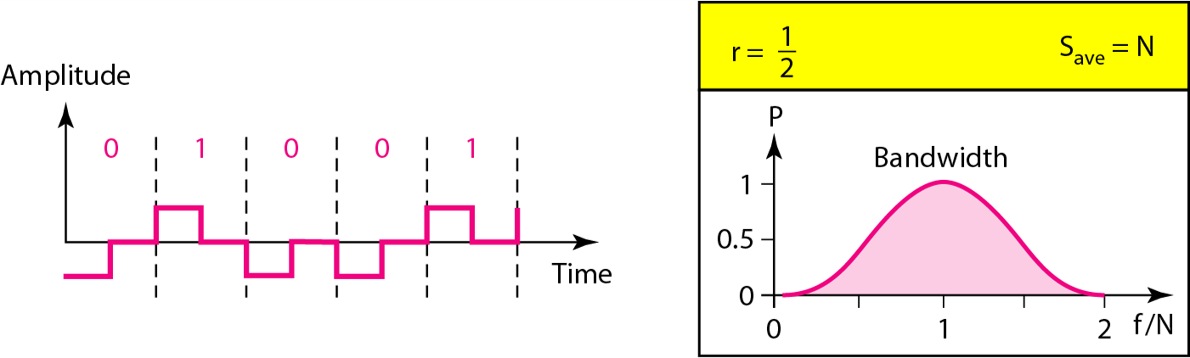
\includegraphics[width=0.9\columnwidth]{bab5/Picture7}
  \caption{Implementation of BFSK}
  \label{fig5:7}
\end{figure}

\subsection*{Multilevel FSK}
Multilevel modulation (MFSK) is not uncommon with the FSK method. We can use more than two frequencies. For example, we can use four different frequenciesfIJ2,!3, and 14 to send 2 bits at a time. To send 3 bits at a time, we can use eight frequencies. And so on. However, we need to remember that the frequencies need to be 2~1 apart. For the proper operation of the modulator and demodulator, it can be shown that the minimum value of 2~lneeds to be S. We can show that the bandwidth with d =0 is

\begin{equation}
  B = (1 + d) \times S + (L - 1)2\Delta f
\end{equation}

\begin{equation}
  B = L \times S
\end{equation}

\begin{example}
  We need to send data 3 bits at a time at a bit rate of 3 Mbps. The carrier frequency is 10 MHz. Calculate the number of levels (different frequencies), the baud rate, and the bandwidth
\end{example}

\begin{solution}
  We can have L =23 =8. The baud rate is S =3 MHz/3 =1000 Mbaud. This means that the carrier frequencies must be 1 MHz apart (211f =1 MHz). The bandwidth is B =8 x 1000 =8000. Figure 5.8 shows the allocation of frequencies and bandwidth.
\end{solution}

\begin{figure}
  \centering
  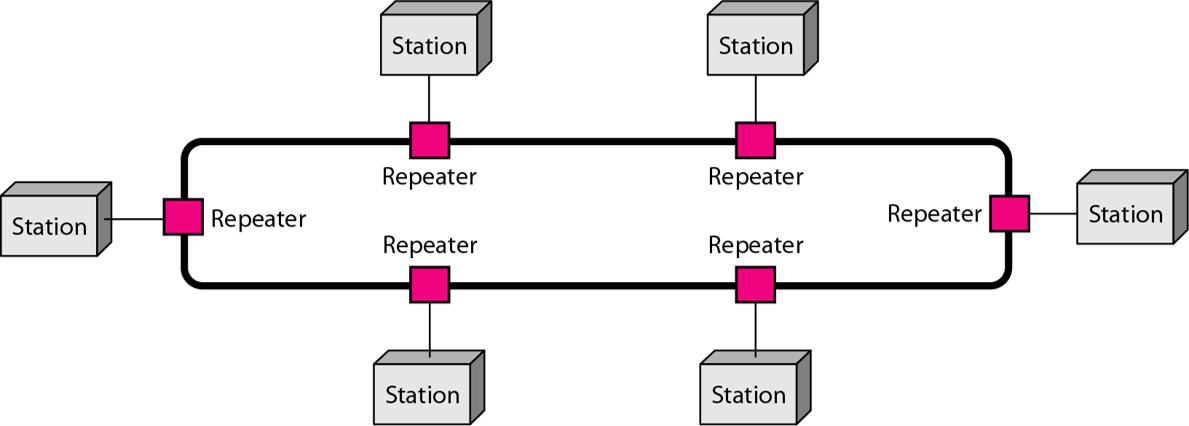
\includegraphics[width=0.9\columnwidth]{bab5/Picture8.png}
  \caption{Bandwidth ofMFSK used in Example 5.6}
  \label{fig5:8}
\end{figure}

\subsection{Phase Shift Keying}
In phase shift keying, the phase of the carrier is varied to represent two or more different signal elements. Both peak amplitude and frequency remain constant as the phase changes. Today, PSK is more common than ASK or FSK. However, we will see Sh0l1ly that QAM, which combines ASK and PSK, is the dominant method of digital-to-analog modulation

\subsection*{Binary PSK (BPSK)}
The simplest PSK is binary PSK, in which we have only two signal elements, one with a phase of 0°, and the other with a phase of 180°. Figure 5.9 gives a conceptual view of PSK. Binary PSK is as simple as binary ASK with one big advantage-it is less susceptible to noise. In ASK, the criterion for bit detection is the amplitude of the signal; in PSK, it is the phase. Noise can change the amplitude easier than it can change the phase. In other words, PSK is less susceptible to noise than ASK. PSK is superior to FSK because we do not need two carrier signals.

\begin{figure}
  \centering
  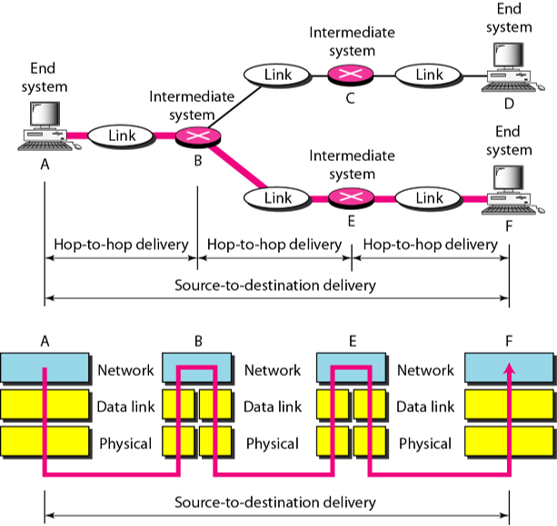
\includegraphics[width=0.9\columnwidth]{bab5/Picture9.png}
  \caption{Binary phase shift keying}
  \label{fig5:9}
\end{figure}

Bandwidth Figure 5.9 also shows the bandwidth for BPSK. The bandwidth is the same as that for binary ASK, but less than that for BFSK. No bandwidth is wasted for separating two carrier signals.

\textbf{Implementation} The implementation of BPSK is as simple as that for ASK. The reason is that the signal element with phase 180° can be seen as the complement of the signal element with phase 0°. This gives us a clue on how to implement BPSK. We use the same idea we used for ASK but with a polar NRZ signal instead of a unipolar NRZ signal, as shown in Figure 5.10. The polar NRZ signal is multiplied by the carrier frequency; the 1 bit (positive voltage) is represented by a phase starting at 0°; the abit (negative voltage) is represented by a phase starting at 180°.

\begin{figure}
  \centering
  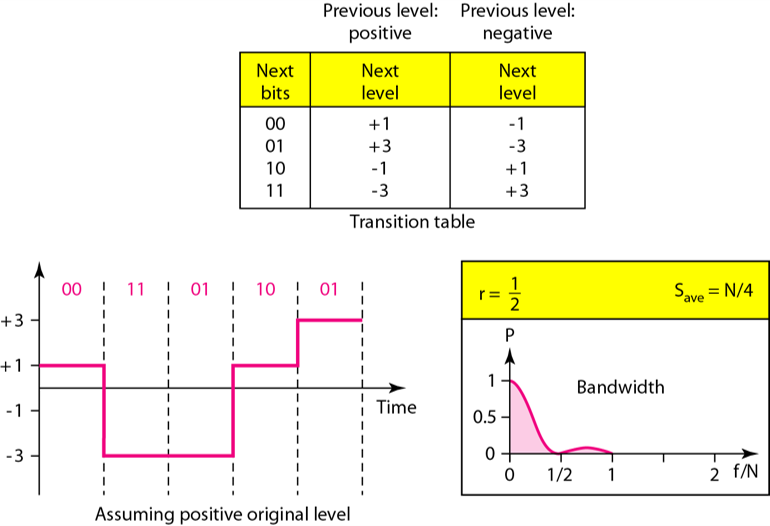
\includegraphics[width=0.9\columnwidth]{bab5/Picture10.png}
  \caption{Implementation of BASK}
  \label{fig5:10}
\end{figure}

\subsection*{Quadrature PSK (QPSK)}
The simplicity of BPSK enticed designers to use 2 bits at a time in each signal element, thereby decreasing the baud rate and eventually the required bandwidth. The scheme is called quadrature PSK or QPSK because it uses two separate BPSK modulations; one is in-phase, the other quadrature (out-of-phase). The incoming bits are first passed through a serial-to-parallel conversion that sends one bit to one modulator and the next bit to the other modulator. If the duration of each bit in the incoming signal is T, the duration of each bit sent to the corresponding BPSK signal is 2T. This means that the bit to each BPSK signal has one-half the frequency of the original signal. Figure 5.11 shows the idea.

The two composite signals created by each multiplier are sine waves with the same frequency, but different phases. When they are added, the result is another sine wave, with one of four possible phases: 45°, -45°, 135°, and -135°. There are four kinds of signal elements in the output signal (L = 4), so we can send 2 bits per signal element (r =2)

\begin{figure}[htbp]
  \centering
  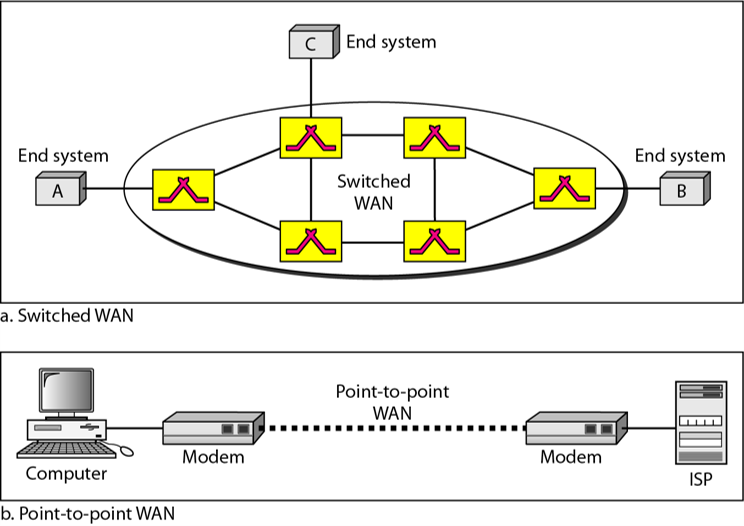
\includegraphics[width=0.9\columnwidth]{bab5/Picture11.png}
  \caption{QPSK and its implementation}
  \label{fig5:11}
\end{figure}

\begin{example}
  Find the bandwidth for a signal transmitting at 12 Mbps for QPSK. The value of d = 0.
\end{example}

\begin{solution}
  For QPSK, 2 bits is carried by one signal element. This means that r =2. So the signal rate (baud rate) is S =N x (lIr) =6 Mbaud. With a value of d =0, we have B =S =6 MHz.
\end{solution}

\subsection*{Constellation Diagram}
A constellation diagram can help us define the amplitude and phase of a signal element, particularly when we are using two carriers (one in-phase and one quadrature), The diagram is useful when we are dealing with multilevel ASK, PSK, or QAM (see next section). In a constellation diagram, a signal element type is represented as a dot. The bit or combination of bits it can carry is often written next to it.

A constellation diagram can help us define the amplitude and phase of a signal element, particularly when we are using two carriers (one in-phase and one quadrature), The diagram is useful when we are dealing with multilevel ASK, PSK, or QAM (see next section). In a constellation diagram, a signal element type is represented as a dot. The bit or combination of bits it can carry is often written next to it.

\begin{figure}[htbp]
  \centering
  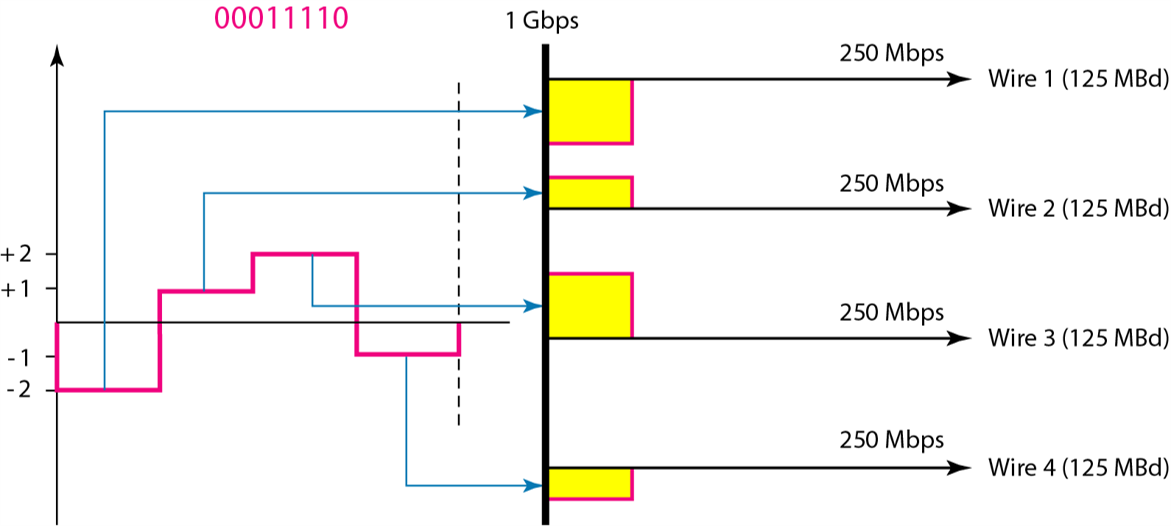
\includegraphics[width=0.9\columnwidth]{bab5/Picture12.png}
  \caption{Concept ofa constellation diagram}
  \label{fig5:12}
\end{figure}

\begin{example}
  Show the constellation diagrams for an ASK (OOK), BPSK, and QPSK signals.
\end{example}

\begin{solution}
  Figure 5.13 shows the three constellation diagrams.

  \begin{figure}
    \centering
    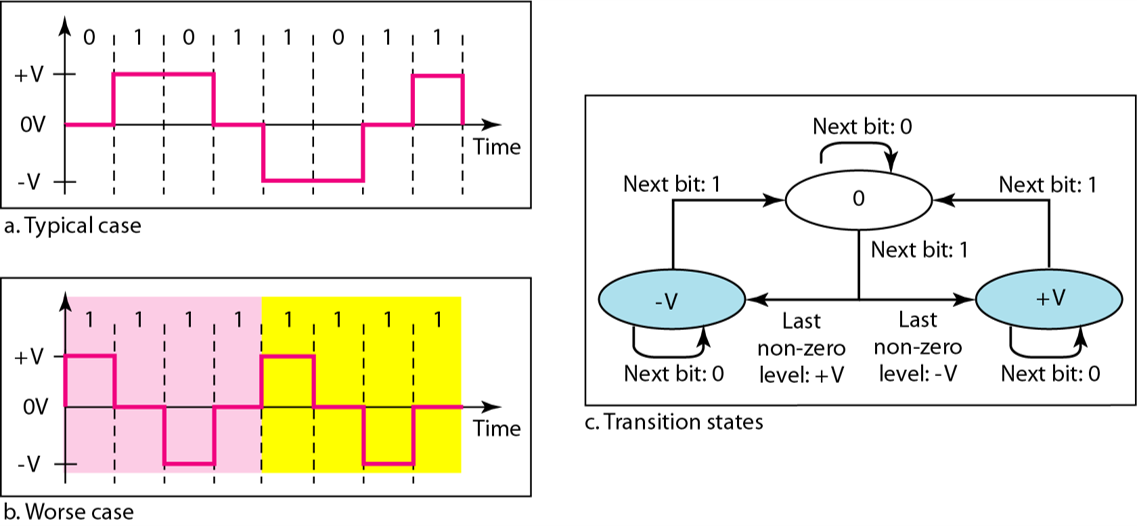
\includegraphics[width=0.9\columnwidth]{bab5/Picture13.png}
    \caption{Three constellation diagrams}
    \label{fig5:13}
  \end{figure}

  Let us analyze each case separately:
  \begin{itemize}
    \item[a.] For ASK, we are using only an in-phase carrier. Therefore, the two points should be on the X axis. Binary 0 has an amplitude of 0 V; binary 1 has an amplitude of 1 V (for example). The points are located at the origin and at 1 unit.
    \item[b.] BPSK also uses only an in-phase carrier. However, we use a polar NRZ signal for modulation. It creates two types of signal elements, one with amplitude 1 and the other with amplitude -1. This can be stated in other words: BPSK creates two different signal elements, one with amplitude I V and in phase and the other with amplitude 1V and 1800 out of phase.
    \item[c.] QPSK uses two carriers, one in-phase and the other quadrature. The point representing 11 is made of two combined signal elements, both with an amplitude of 1 V. One element is represented by an in-phase carrier, the other element by a quadrature carrier. The amplitude of the final signal element sent for this 2-bit data element is 2112, and the phase is 45°. The argument is similar for the other three points. All signal elements have an amplitude of 2112, but their phases are different (45°, 135°, -135°, and -45°). Of course, we could have chosen the amplitude of the carrier to be 1/(21/2) to make the final amplitudes 1V.
  \end{itemize}
\end{solution}

\subsection{Quadrature Amplitude Modulation}
PSK is limited by the ability of the equipment to distinguish small differences in phase. This factor limits its potential bit rate. So far, we have been altering only one of the three characteristics of a sine wave at a time; but what if we alter two? Why not combine ASK and PSK? The idea of using two carriers, one in-phase and the other quadrature, with different amplitude levels for each carrier is the concept behind quadrature amplitude modulation (QAM). Quadrature amplitude modulation is a combination of ASK and PSK.

The possible variations of QAM are numerous. Figure 5.14 shows some of these schemes. Figure 5.14a shows the simplest 4-QAM scheme (four different signal element types) using a unipolar NRZ signal to modulate each carrier. This is the same mechanism we used for ASK (OOK). Part b shows another 4-QAM using polar NRZ, but this is exactly the same as QPSK. Part c shows another QAM-4 in which we used a signal with two positive levels to modulate each of the two carriers. Finally, Figure 5.14d shows a 16-QAM constellation of a signal with eight levels, four positive and four negative

\begin{figure}
  \centering
  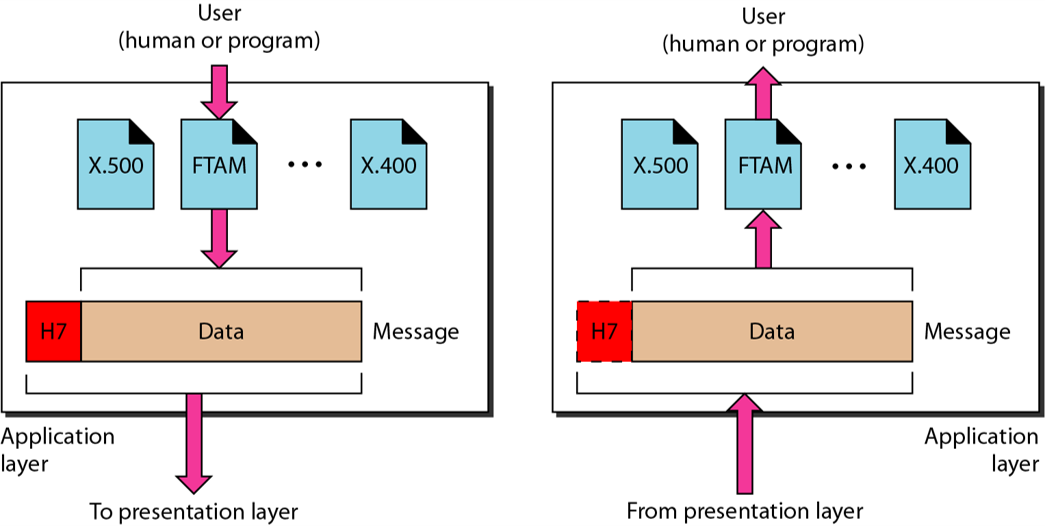
\includegraphics[width=0.9\columnwidth]{bab5/Picture14.png}
  \caption{Constellation diagramsfor some QAMs}
  \label{fig5:14}
\end{figure}

\subsection*{Bandwidth for QAM}
The minimum bandwidth required for QAM transmission is the same as that required for ASK and PSK transmission. QAM has the same advantages as PSK over ASK.

\section{Konversi Analog-to-analog}
Analog-to-analog conversion, or analog modulation, is the representation of analog information by an analog signal. One may ask why we need to modulate an analog signal; it is already analog. Modulation is needed if the medium is bandpass in nature or if only a bandpass channel is available to us. An example is radio. The government assigns a narrow bandwidth to each radio station. The analog signal produced by each station is a low-pass signal, all in the same range. To be able to listen to different stations, the low-pass signals need to be shifted, each to a different range.

Analog-to-analog conversion can be accomplished in three ways: amplitude modulation (AM), frequency modulation (FM), and phase modulation (PM). FM and PM are usually categorized together. See Figure 5.15.

\begin{figure}
  \centering
  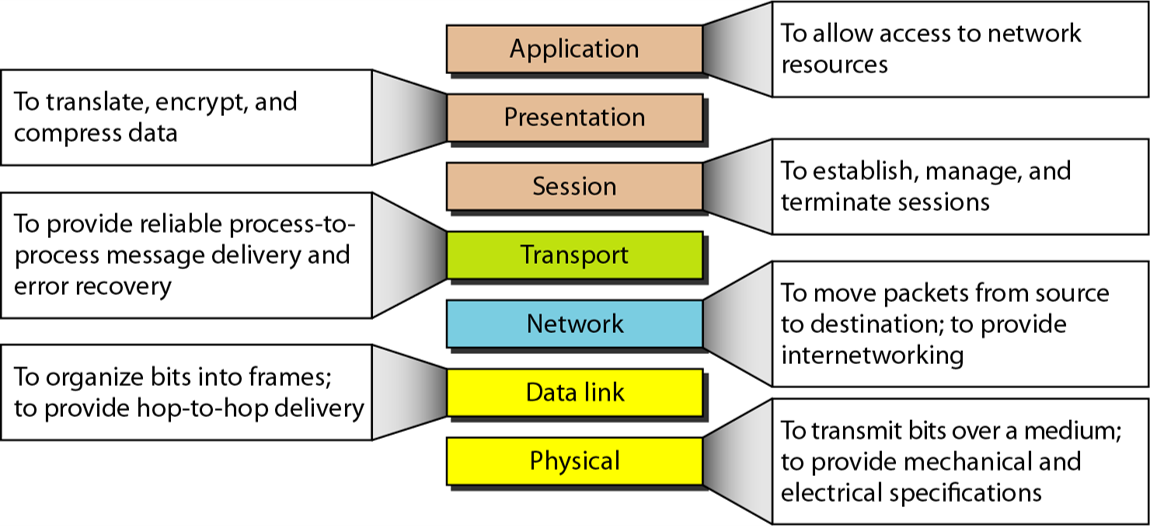
\includegraphics[width=0.9\columnwidth]{bab5/Picture15.png}
  \caption{Types of analog-to-analog modulation}
  \label{fig5:15}
\end{figure}

\subsection{Amplitude Modulation}
In AM transmission, the carrier signal is modulated so that its amplitude varies with the changing amplitudes of the modulating signal. The frequency and phase of the carrier remain the same; only the amplitude changes to follow variations in the information. Figure 5.16 shows how this concept works. The modulating signal is the envelope ofthe carrier

\begin{figure}
  \centering
  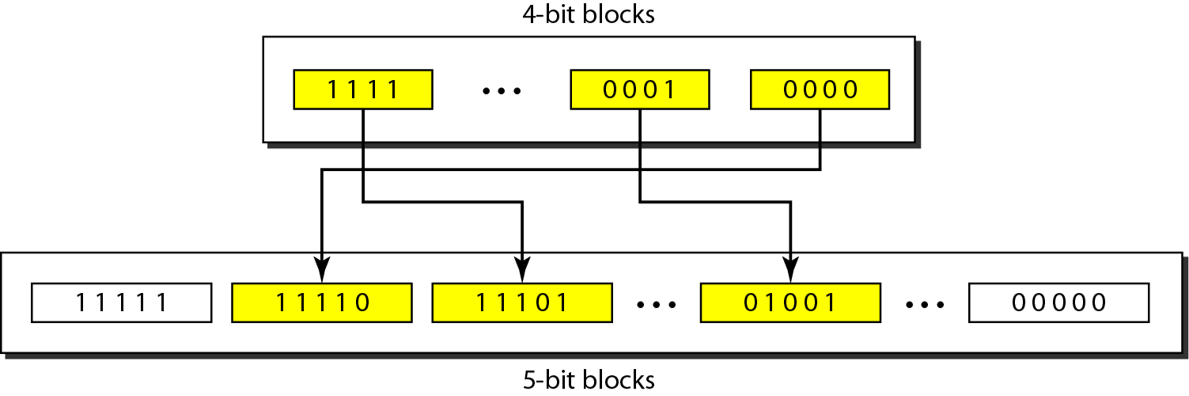
\includegraphics[width=0.9\columnwidth]{bab5/Picture16.png}
  \caption{Amplitude modulation}
  \label{fig5:16}
\end{figure}

As Figure 5.16 shows, AM is normally implemented by using a simple multiplier because the amplitude of the carrier signal needs to be changed according to the amplitude of the modulating signal.

\subsection*{AM Bandwidth}
Figure 5.16 also shows the bandwidth of an AM signal. The modulation creates a bandwidth that is twice the bandwidth of the modulating signal and covers a range centered on the carrier frequency. However, the signal components above and below the carrier frequency carry exactly the same information. For this reason, some implementations discard one-half of the signals and cut the bandwidth in half. The total bandwIdth required for AM can be determined from the bandwidth of the audio signal: 

\begin{equation}
  B_{AM} =2B
\end{equation}

\subsection*{Standard Balldwidth Allocatioll for AM Radio}
The bandwidth of an audio signal (speech and music) is usually 5 kHz. Therefore, an AM radio station needs a bandwidth of 10kHz. In fact, the Federal Communications Commission (FCC) allows 10 kHz for each AM station.

AM stations are allowed carrier frequencies anywhere between 530 and 1700 kHz (1.7 MHz). However, each station's carrier frequency must be separated from those on either side of it by at least 10 kHz (one AM bandwidth) to avoid interference. If one station uses a carrier frequency of 1100 kHz, the next station's carrier frequency cannot be lower than 1110 kHz (see Figure 5.17)

\begin{figure}
  \centering
  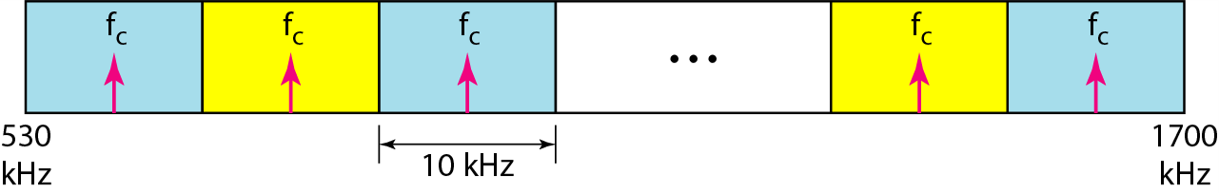
\includegraphics[width=0.9\columnwidth]{bab5/Picture17.png}
  \caption{AM band allocation}
  \label{fig5:17}
\end{figure}

\subsection{Frequency Modulation}
In FM transmission, the frequency of the carrier signal is modulated to follow the changing voltage level (amplitude) of the modulating signal. The peak amplitude and phase of the carrier signal remain constant, but as the amplitude of the information signal changes, the frequency of the carrier changes correspondingly. Figure 5.18 shows the relationships of the modulating signal, the carrier signal, and the resultant FM signal. 

As Figure 5.18 shows, FM is nOimalIy implemented by using a voltage-controlled oscillator as with FSK. The frequency of the oscillator changes according to the input voltage which is the amplitude of the modulating signal.

\subsection*{FM Bandwidth}
Figure 5.18 also shows the bandwidth of an FM signal. The actual bandwidth is difficult to determine exactly, but it can be shown empirically that it is several times that of the analog signal or $2(1 + \beta)B$ where is a factor depends on modulation technique with a common value of 4. The total bandwidth required for FM can be determined from the bandwidth of the audio signal.

\begin{equation}
  B_{FM} =2(1 + \beta)B
\end{equation}

\begin{figure}
  \centering
  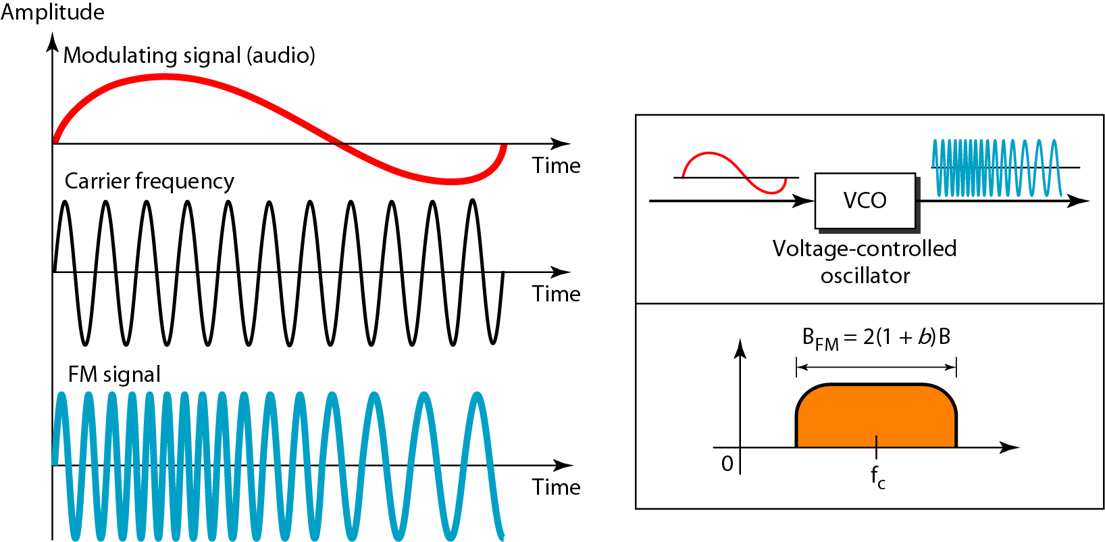
\includegraphics[width=0.9\columnwidth]{bab5/Picture18.png}
  \caption{Frequency modulation}
  \label{fig5:18}
\end{figure}

\subsection*{Standard Bandwidth Allocation for FM Radio}
The bandwidth of an audio signal (speech and music) broadcast in stereo is almost 15 kHz. The FCC allows 200 kHz (0.2 MHz) for each station. This mean = 4 with some extra guard band. FM stations are allowed carrier frequencies anywhere between 88 and 108 MHz. Stations must be separated by at least 200 kHz to keep their bandwidths from overlapping. To create even more privacy, the FCC requires that in a given area, only alternate bandwidth allocations may be used. The others remain unused to prevent any possibility of two stations interfering with each other. Given 88 to 108 MHz as a range, there are 100 potential PM bandwidths in an area, of which 50 can operate at anyone time. Figure 5.19 illustrates this concept.

\begin{figure}
  \centering
  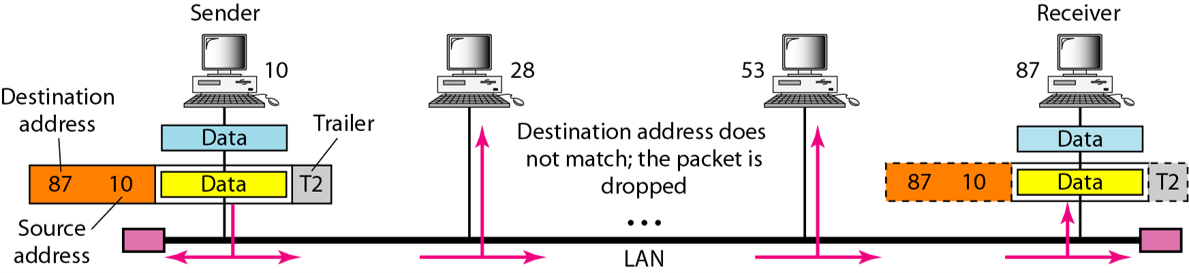
\includegraphics[width=0.9\columnwidth]{bab5/Picture19.png}
  \caption{FM band allocation}
  \label{fig5:19}
\end{figure}

\subsection{Phase Modulation}
In PM transmission, the phase of the carrier signal is modulated to follow the changing voltage level (amplitude) of the modulating signal. The peak amplitude and frequency of the carrier signal remain constant, but as the amplitude of the information signal changes, the phase of the carrier changes correspondingly. It can proved mathematically (see Appendix C) that PM is the same as FM with one difference. In FM, the instantaneous change in the carrier frequency is proportional to the amplitude of the modulating signal; in PM the instantaneous change in the carrier frequency is proportional to the derivative of the amplitude of the modulating signal. Figure 5.20 shows the relationships of the modulating signal, the carrier signal, and the resultant PM signal.

\begin{figure}
  \centering
  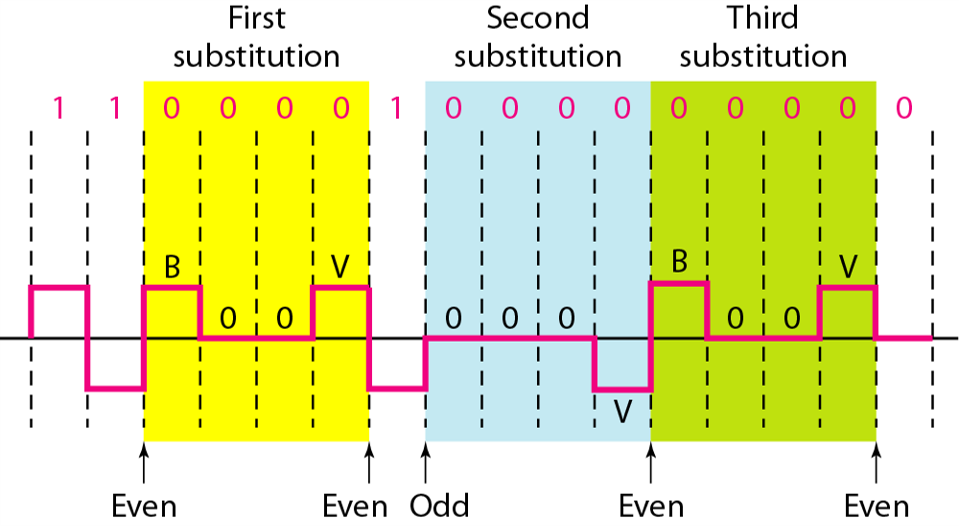
\includegraphics[width=0.9\columnwidth]{bab5/Picture20.png}
  \caption{Phase modulation}
  \label{fig5:20}
\end{figure}

As Figure 5.20 shows, PM is normally implemented by using a voltage-controlled oscillator along with a derivative. The frequency of the oscillator changes according to the derivative of the input voltage which is the amplitude of the modulating signal.

\subsection*{PM Bandwidth}
Figure 5.20 also shows the bandwidth of a PM signal. The actual bandwidth is difficult to determine exactly, but it can be shown empirically that it is several times that of the analog signal. Although, the formula shows the same bandwidth for FM and PM, the value of is lower in the case of PM (around 1 for narrowband and 3 for wideband). The total bandwidth required for PM can be determined from the bandwidth and maximum amplitude of the modulating signal:

\begin{equation}
  B_{PM} = 2(1 + \beta)B
\end{equation}


\section{Ringkasan}
\begin{itemize}
  \item[$\odot$] Digital-to-analog conversion is the process of changing one of the characteristics of an analog signal based on the information in the digital data
  \item[$\odot$] Digital-to-analog conversion can be accomplished in several ways: amplitude shift keying (ASK), frequency shift keying (FSK), and phase shift keying (PSK). Quadrature amplitude modulation (QAM) combines ASK and PSK.
  \item[$\odot$] In amplitude shift keying, the amplitude of the carrier signal is varied to create signal elements. Both frequency and phase remain constant while the amplitude changes.
  \item[$\odot$] In frequency shift keying, the frequency of the carrier signal is varied to represent data. The frequency of the modulated signal is constant for the duration of one signal element, but changes for the next signal element if the data element changes. Both peak amplitude and phase remain constant for all signal elements.
  \item[$\odot$] In phase shift keying, the phase of the carrier is varied to represent two or more different signal elements. Both peak amplitude and frequency remain constant as the phase changes.
  \item[$\odot$] A constellation diagram shows us the amplitude and phase of a signal element, particularly when we are using two carriers (one in-phase and one quadrature).
  \item[$\odot$] Quadrature amplitude modulation (QAM) is a combination of ASK and PSK. QAM uses two carriers, one in-phase and the other quadrature, with different amplitude levels for each carrier.
  \item[$\odot$] Analog-to-analog conversion is the representation of analog information by an analog signal. Conversion is needed if the medium is bandpass in nature or if only a bandpass bandwidth is available to us
  \item[$\odot$] Analog-to-analog conversion can be accomplished in three ways: amplitude modulation (AM), frequency modulation (FM), and phase modulation (PM).
  \item[$\odot$] In AM transmission, the carrier signal is modulated so that its amplitude varies with the changing amplitudes of the modulating signal. The frequency and phase of the carrier remain the same; only the amplitude changes to follow variations in the information.
  \item[$\odot$] In PM transmission, the frequency of the carrier signal is modulated to follow the changing voltage level (amplitude) of the modulating signal. The peak amplitude and phase of the carrier signal remain constant, but as the amplitude of the information signal changes, the frequency of the carrier changes correspondingly.
  \item[$\odot$] In PM transmission, the phase of the carrier signal is modulated to follow the changing voltage level (amplitude) of the modulating signal. The peak amplitude and frequency of the carrier signal remain constant, but as the amplitude of the information signal changes, the phase of the carrier changes correspondingly.
\end{itemize}

\section{Latihan}

\subsection*{Pertanyaan ulasan}

\begin{enumerate}
  \item Define analog transmission.
  \item Define carrier signal and its role in analog transmission
  \item Define digital-to-analog conversion.
  \item Which characteristics of an analog signal are changed to represent the digital signal in each of the following digital-to-analog conversion?
  \item Which of the four digital-to-analog conversion techniques (ASK, FSK, PSK or QAM) is the most susceptible to noise? Defend your answer.
  \item Define constellation diagram and its role in analog transmission.
  \item What are the two components of a signal when the signal is represented on a con- . stellation diagram? Which component is shown on the horizontal axis? Which is shown on the vertical axis?
  \item Define analog-to-analog conversion?
  \item Which characteristics of an analog signal are changed to represent the lowpass analog signal in each of the following analog-to-analog conversions?
  \item Which of the three analog-to-analog conversion techniques (AM, FM, or PM) is the most susceptible to noise? Defend your answer
\end{enumerate}

\subsection*{Latihan}
\begin{enumerate}[resume]
  \item Calculate the baud rate for the given bit rate and type of modulation.
  \item Calculate the bit rate for the given baud rate and type of modulation.
  \item What is the number of bits per baud for the following techniques?
  \item Draw the constellation diagram for the following:
  \item Draw the constellation diagram for the following cases. Find the peak amplitude value for each case and define the type of modulation (ASK, FSK, PSK, or QAM). The numbers in parentheses define the values of I and Q respectively.
  \item How many bits per baud can we send in each of the following cases if the signal constellation has one of the following number of points?
  \item What is the required bandwidth for the following cases if we need to send 4000 bps? Let d = 1.
  \item The telephone line has 4 KHz bandwidth. What is the maximum number of bits we can send using each of the following techniques? Let d = 0.
  \item A corporation has a medium with a I-MHz bandwidth (lowpass). The corporation needs to create 10 separate independent channels each capable of sending at least 10 Mbps. The company has decided to use QAM technology. What is the minimum number of bits per baud for each channel? What is the number of points in the constellation diagram for each channel? Let d = 0.
  \item A cable company uses one of the cable TV channels (with a bandwidth of 6 MHz) to provide digital communication for each resident. What is the available data rate for each resident if the company uses a 64-QAM technique?
  \item Find the bandwidth for the following situations if we need to modulate a 5-KHz voice.
  \item Find the total number of channels in the corresponding band allocated by FCC.
\end{enumerate}